\section{Asteroid Identification}
\label{sec:processing}

The calibrated images and source catalogs support two complementary
paths (Figure~\ref{fig:workflow}). The first associates detections with
predicted positions of known asteroids. The second identifies
consistent motion among repeated detections and then removes links
attributed to known objects. Both retain the image and observation
time associated with each measurement.

\begin{figure}[tbp]
\centering
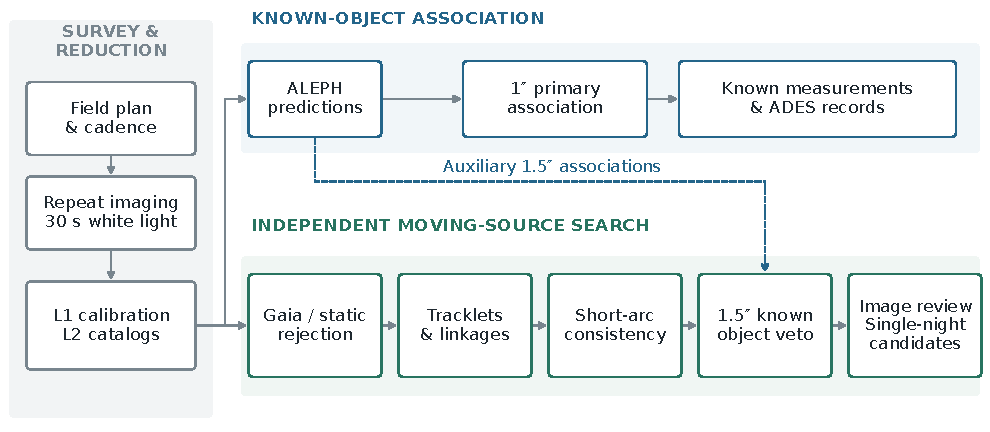
\includegraphics[width=\linewidth]{fig02_workflow.pdf}
\caption{The observing and identification sequence. Repeated white-light
imaging produces calibrated images and source catalogs. The upper branch
associates sources with ALEPH predictions to form the primary
$1\asec$ known-object sample. The moving-source branch constructs
tracklets and links after stationary-source rejection, tests short-arc
consistency, and removes links identified by the auxiliary $1.5\asec$
known-object associations. The dashed connection supplies those
identities after motion linking. Image inspection selects the
single-night candidates. L1 and L2 denote calibrated images and
source catalogs, respectively; ADES is the Astrometric Data Exchange
Standard.}
\label{fig:workflow}
\end{figure}

\label{sec:known_method}
Topocentric directions of known asteroids are calculated at the exposure
midpoint using the Lowell \texttt{astorb} catalog
\citep{Moskovitz2022Astorb} and ALEPH \citep{PenaZamudioFuentes2021ALEPH},
with the observing position at Xinglong. Predictions with $V<22.5$
within the image are compared with detected sources. The primary sample
uses the nearest association within $1.0\asec$. An auxiliary
$1.5\asec$ match supplies identities for known-object subtraction and
for the linkage assessment below. The magnitude criterion sets the
prediction limit. Association relies on angular separation, with no
restrictive cut on the difference between predicted $V$ and observed
\gaper, which are on different photometric scales. Sparse matches in
the distant-orbit region receive additional checks for apparent motion
in neighboring images (Section~\ref{sec:known_population}).

The reference orbit catalog contains asteroids. Cometary detections
therefore remain in the independent moving-source sample until
identified separately, as illustrated by C/2025~Y1 in
Section~\ref{sec:candidates}. Astrometric measurements can be written
in ADES format for subsequent reporting.

\label{sec:motion_method}
The independent search begins with repeated observations of a field.
Gaia matches, stationary-source patterns, and detections near image
edges are removed before two-detection tracklets are constructed.
Tracklets with common endpoints are joined into links with at least
three measurements. The adopted angular-rate interval is
$3$--$63$~\rateunit. Tracklet members may differ by at most 1~mag;
linked tracklets must agree within 5~\rateunit\ in rate and
$10^\circ$ in direction. These criteria select a coherent angular
trajectory over a night.

The resulting chains are tested with a heliocentric short-arc
calculation. Heliocentric transformations provide a useful framework
for linking moving-source detections \citep{Holman2018}. Here, a
solar two-body Lambert solution \citep{Izzo2015} is evaluated for
eight equal-endpoint heliocentric-distance hypotheses,
$r=1.3,1.7,\ldots,4.1$~au. Solutions for the full chain and tracklet
subsets are compared by their angular RMS. Accepted solutions have
observer distances above 0.02~au at both endpoints and a final-epoch
heliocentric speed below 35~km~s$^{-1}$. The distance grid specifies
the Lambert endpoints, while the fitted orbit follows from the
trajectory solution. Appendix~\ref{app:shortarc} describes the
interpretation of these short-arc fits.

Links with successful fits and no auxiliary known-asteroid association
among their members form the automatic candidate list. Time-ordered
image sequences are inspected for source morphology, blending,
artifacts, and displacement across the images. The retained sample
consists of links with coherent motion supported by the image
sequence. Automatic and image-inspected samples are reported with
their respective observing coverage in Section~\ref{sec:candidates}.

\label{sec:retention_method}
Known asteroids provide an empirical measure of how often repeated
detections are assembled into links. An eligible object--night consists
of at least three distinct science exposures containing detections
associated with one identity within $1.5\asec$, with a predicted
first-to-last angular rate of $3$--$63$~\rateunit. It is recovered
when a link has members in at least three distinct exposures, all
uniquely associated with that identity. Links are examined before
known-object subtraction.
We define the conditional linkage retention as
\begin{equation}
R_{\rm cond}=\frac{N_{\rm linked}}{N_{\rm eligible}},
\label{eq:retention}
\end{equation}
where both counts use the first-year exposure selection and the same
observing-night definition. The evaluated observations comprise
\yrNRetExposures\ exposures on \yrNRetNights\ nights for which the
motion-search outputs are available. This statistic measures linking
given catalog detection, adequate sampling, and an angular rate within
the search interval. It reflects source rejection, field grouping,
and construction of the links available before known-object subtraction.
